\section{Bending the round end}
\label{sec:bending}

The collar has produced the round leaves needed for the model of
Section~\ref{sec:model}. We now lower their tangential tensor trace
$2v/r$ from $2$ to zero. The angular mass function is not discarded:
its mean will become the ADM energy, while its other modes are smoothed
by heat evolution. The trace-free correction from
Lemma~\ref{lem:obstruction} removes the associated angular momentum.
The increasing mass term already present in the collar then absorbs
all remaining constraint errors.

There are two radial scales. We begin reducing $v/r$ at a radius
comparable to $R$, but postpone its final cutoff to the annulus
$R^2\leq r\leq2R^2$.
By then $v$ and its scaled derivatives are small, so the final cutoff
is smooth without a singular estimate involving $1/v$. Heat evolution
is activated before either change, while $v=r$.

\begin{lemma}[Angular heat evolution]\label{lem:sphere-heat}
Suppose $f_*\in C^\infty(\Sph)$ has average $m$ and vanishing first
spherical harmonic. There are smooth functions $f(t,\omega)$ and
trace-free symmetric tensors $\mathcal T(t,\omega)$, for $t\geq0$,
such that
\[
 \partial_t f=\Delta_\sigma f,\qquad f(0,\cdot)=f_*,\qquad
 \avg{f(t,\cdot)}=m,\qquad
 \diver_\sigma\mathcal T=\mathrm d_{\Sph}f.
\]
Every fixed-order angular and time derivative of $f$ and $\mathcal T$
is bounded uniformly for $t\geq0$. More precisely, for all nonnegative
integers $a,b$,
\[
 \|\nabla_\sigma^a\partial_t^b(f-m)\|_{L^\infty}
 +\|\nabla_\sigma^a\partial_t^b\mathcal T\|_{L^\infty}
 \leq C_{a,b}e^{-6t}.
\]
\end{lemma}

\begin{proof}
Let $f_{*,\ell}$ be the projection onto the degree-$\ell$ spherical
harmonics and put $\lambda_\ell=\ell(\ell+1)$. Define
\begin{equation}\label{eq:spherical-series}
 \begin{split}
 f(t)&=m+\sum_{\ell\geq2}e^{-\lambda_\ell t}f_{*,\ell},\\
 \psi(t)&=\sum_{\ell\geq2}
       \frac{e^{-\lambda_\ell t}}{1-\lambda_\ell/2}f_{*,\ell},
 \qquad
 \mathcal T=(\nabla_\sigma^2\psi)^{\TF}.
 \end{split}
\end{equation}
The degree-one term is absent by hypothesis. For each $t$, this is
the inverse constructed in Lemma~\ref{lem:obstruction}, applied to
$f(t)$; hence $\diver_\sigma\mathcal T=\mathrm d_{\Sph}f$.
The complete orthogonal decomposition into spherical harmonics
converges here with all fixed-order derivatives, even at $t=0$, because
the initial function is smooth. Explicitly, repeated integration by
parts gives
\[
 \|f_{*,\ell}\|_{L^2}
   \leq \lambda_\ell^{-N}\|\Delta_\sigma^N f_*\|_{L^2}
   \qquad (\ell\geq2)
\]
for every $N$. The $C^a$ norm of a degree-$\ell$ harmonic is bounded
by a polynomial in $\lambda_\ell$ times its $L^2$ norm. One can see
this directly from the addition formula, whose diagonal value is
$(2\ell+1)/(4\pi)$, and repeated differentiation by rotation fields:
these preserve the eigenspace, have $L^2$ operator norm at most
$\sqrt{\lambda_\ell}$ there, and span the tangent spaces of the sphere.
These polynomial bounds, with $N$ arbitrarily large, justify all
differentiations, including time differentiation and the two
derivatives defining $\mathcal T$. Since $\lambda_\ell\geq6$ for
$\ell\geq2$, the same summation gives the asserted exponential
decay. Preservation of the average is immediate.
\end{proof}

We apply Lemma~\ref{lem:sphere-heat} with the balanced aspect $f_*$
and $m=m_B$. All constants below may depend on this smooth aspect
and on fixed cutoff profiles, but not on the large parameter $R$.
We use $C_*$ for a positive bound that may increase from line to line,
to distinguish such constants from the constraint quantity $C$.

The two coefficients in the bending prescription can be read from the
round constraints. To see this, consider first the region after the
joining annulus, where the added normal term has disappeared. Take
$\gamma=r^2\sigma$, $L=v'$, $\eta=0$, and set $A=1+v^2$ and
$u^2=A-2F/r$, temporarily leaving $F$ and $\tau$ undetermined.
Replacing $u^2$ by $A$ in the angular coefficients, the terms to cancel
in the scalar and tangential momentum constraints are, respectively,
\[
 \frac{2\partial_rF}{r^2}-\frac{\Delta_\sigma F}{r^3A},
 \qquad
 \diver_\gamma\tau-\frac{v'-v/r}{rA}\mathrm d_{\Sph}F.
\]
The first expression suggests taking $F=f(t(r),\omega)+c_R(r)$
with $t'=1/(2rA)$; the radial padding then contributes only its positive
mass derivative. For the second, since
$\diver_\sigma\mathcal T=\mathrm d_{\Sph}f$ and
$\diver_\gamma=r^{-2}\diver_\sigma$ on covariant sphere tensors,
the coefficient of $\mathcal T$ must be $r(v'-v/r)/A$.
This calculation chooses the formulas. The proof below retains the
exact coefficients and all quadratic terms, and starts heat evolution
before changing $v/r$ to handle the joining annulus.

\begin{lemma}[Outer bending]\label{lem:bending}
Let $f,\mathcal T$ be the heat evolution and trace-free tensors of
Lemma~\ref{lem:sphere-heat}, with initial value the balanced aspect
$f_*$. For all sufficiently large $R$, there are smooth radial
functions $t:[3R,\infty)\to[0,\infty)$,
$\beta:[3R,\infty)\to[0,1]$ and $v:[3R,\infty)\to[0,\infty)$
such that the round data at the outer edge of the collar extend
smoothly to $r\geq3R$, satisfy the dominant energy condition,
and have the form
\begin{equation}\label{eq:outer-data}
 \begin{gathered}
 G=u^{-2}\mathrm dr^2+r^2\sigma,\qquad
 u^2=1+v^2-\frac{2F}{r},\qquad
 F=f(t(r),\omega)+c_R(r),\\
 k(N,N)=v'+\frac{\beta}{r^2},\qquad
 k(N,\cdot)|_{T\Sph}=0,\qquad
 k_T=\frac vr\gamma+\tau,\qquad \gamma=r^2\sigma,\\
 \tau=\frac{r(v'-v/r)}{1+v^2}\mathcal T(t(r),\omega),
 \qquad N=u\partial_r.
 \end{gathered}
\end{equation}
Here $0\leq v\leq r$, $v=r$ through $6R$, and $v=0$ for
$r\geq2R^2$. The tensor $k$ vanishes identically for $r\geq2R^2$.
The function $F$ and every fixed-order mixed angular and scaled
radial derivative of $F$ are bounded uniformly in $R$ on $r\geq3R$.
\end{lemma}

\begin{proof}
\emph{The radial profiles.}
Choose fixed smooth functions $\phi,\xi$ on $(0,\infty)$ with
\[
 \begin{array}{lll}
 0<\phi\leq1,&\phi(x)=1\quad(x\leq6),&
             \phi(x)=x^{-3}\quad(x\geq12),\\
 0\leq\xi\leq1,&\xi(x)=1\quad(x\leq1),&
             \xi(x)=0\quad(x\geq2),
 \end{array}
\]
and set
\begin{equation}\label{eq:bending-profile}
 v(r)=r\phi(r/R)\xi(r/R^2),\qquad A=1+v^2.
\end{equation}
We always take $R\geq12$. The profiles can be chosen, and are now
fixed, so that $|(x\partial_x)^j\phi|\leq C_j\phi$ for every fixed
$j$. Away from the final cutoff, logarithmic derivatives of $v$
are therefore bounded by a constant times $v$. On the final cutoff
$R^2\leq r\leq2R^2$, the preceding profile is
$r\phi(r/R)=R^3/r^2=O(R^{-1})$; every scaled derivative of the
product with $\xi(r/R^2)$ is also $O(R^{-1})$. Thus, for every
fixed $j$,
\begin{equation}\label{eq:profile-derivatives}
 |(r\partial_r)^jv|\leq C_j\sqrt A,
 \qquad\text{in particular}\qquad |rv'|\leq C_1\sqrt A.
\end{equation}
This estimate holds across the smooth zero of $v$ without dividing
by $v$.

Choose smooth radial cutoffs $0\leq\zeta,\beta\leq1$, with fixed
profiles in $r/R$, such that
\[
 \zeta=0\quad(r\leq4R),\qquad \zeta=1\quad(r\geq5R),
 \qquad
 \beta=1\ \text{near }3R,\qquad \beta=0\quad(r\geq5R).
\]
Define
\begin{equation}\label{eq:heat-time}
 t(r)=\int_{3R}^r\frac{\zeta(s)}{2sA(s)}\,\mathrm ds,
 \qquad L=v'+\frac{\beta}{r^2},
\end{equation}
and prescribe the data by \eqref{eq:outer-data}. Recall that
$c_R'=r^{-3/2}$ on this entire region. The heat lemma and
$0\leq c_R\leq2R^{-1/2}$ bound $F$ uniformly. In particular,
after increasing $R$,
\begin{equation}\label{eq:lapse-comparison}
 \frac12 A\leq u^2\leq\frac32 A,
 \qquad
 \left|u^{-2}-A^{-1}\right|\leq\frac{C_*}{rA^2}.
\end{equation}
The data are smooth and positive definite. Near $3R$, one has
$v=r$, $t=0$, $\beta=1$, and $\tau=0$. Hence all quantities agree
with the round endpoint of \eqref{eq:collar-data}. The cutoffs are
constant on their designated sides, so this is a smooth match,
including all derivatives at the join.

Figure~\ref{fig:stages} records the order of the modifications. In
particular, heat evolution is fully active and the extra normal entry
has disappeared before $v/r$ begins to decrease.
\begin{figure}[!hb]
\centering
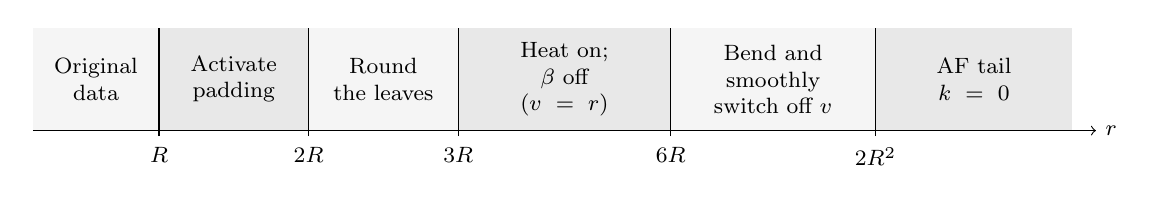
\begin{tikzpicture}[x=1cm,y=1cm,font=\footnotesize]
 \fill[black!4] (0,0) rectangle (1.6,1.3);
 \fill[black!9] (1.6,0) rectangle (3.5,1.3);
 \fill[black!4] (3.5,0) rectangle (5.4,1.3);
 \fill[black!9] (5.4,0) rectangle (8.1,1.3);
 \fill[black!4] (8.1,0) rectangle (10.7,1.3);
 \fill[black!9] (10.7,0) rectangle (13.2,1.3);
 \draw[->] (0,0) -- (13.5,0) node[right] {$r$};
 \foreach \x/\lab in {1.6/R,3.5/2R,5.4/3R,8.1/6R,10.7/2R^2}
  {\draw (\x,-0.07)--(\x,1.3);\node[below] at (\x,-0.09) {$\lab$};}
 \node[align=center,text width=1.5cm] at (0.8,0.65) {Original\\data};
 \node[align=center,text width=1.8cm] at (2.55,0.65) {Activate\\padding};
 \node[align=center,text width=1.8cm] at (4.45,0.65) {Round\\the leaves};
 \node[align=center,text width=2.5cm] at (6.75,0.65) {Heat on;\\$\beta$ off\\($v=r$)};
 \node[align=center,text width=2.4cm] at (9.4,0.65) {Bend and smoothly\\switch off $v$};
 \node[align=center,text width=2.3cm] at (11.95,0.65) {AF tail\\$k=0$};
\end{tikzpicture}
\caption{Order of the end replacement, schematically and not to scale.
The padding cutoff $w$ is one before rounding starts. The heat cutoff
$\zeta$ turns on between $4R$ and $5R$, and $\beta=0$ from $5R$ on,
while $v=r$ through $6R$. The final cutoff of $v$ occurs between $R^2$
and $2R^2$. Heat evolution and the integrable mass increase continue
on the AF tail.}\label{fig:stages}
\end{figure}

The profiles now supply a smooth metric and tensor with the required
end behavior. We must verify their dominant energy condition throughout
the transition, before using the far end to compute mass.

\emph{The exact constraints.}
Here $d=1$, $\widehat\chi=0$, $s=0$, $\eta=0$, and $U=u$.
Substituting in \eqref{eq:constraints} and
\eqref{eq:mass-identity} gives
\begin{equation}\label{eq:round-constraints}
 \begin{split}
 Q&=\frac{2u\beta}{r^3},\\
 C&=\frac vu Q+\frac{2\partial_rF}{r^2}
           -u\Delta_\gamma(u^{-1})-\frac12|\tau|_\gamma^2,\\
 Z&=\diver_\gamma\tau+(L-v/r)\mathrm d_{\Sph}\log u
                       -\tau(B_N,\cdot),
 \qquad B_N=\nabla^\gamma\log u.
 \end{split}
\end{equation}
The first formula follows as well directly from
$H=2u/r$, $p=2v/r$, and $N=u\partial_r$; the terms involving
$v'$ cancel. These are the constraint quantities of the new data,
not prescribed matter fields.

For the energy equation, direct angular differentiation yields
\begin{equation}\label{eq:laplacian-cancellation}
 \begin{split}
 u\Delta_\gamma(u^{-1})
   &=\frac{\Delta_\sigma F}{r^3u^2}
      +\frac{3|\nabla^\sigma F|_\sigma^2}{r^4u^4},\\
 \frac{2\partial_rF}{r^2}
   &=\frac{\zeta\Delta_\sigma F}{r^3A}+\frac{2}{r^{7/2}}.
 \end{split}
\end{equation}
The Laplacian coefficients cancel to the required order. Indeed,
\[
 \frac\zeta A-\frac1{u^2}
   =\frac{\zeta-1}{A}+\left(\frac1A-\frac1{u^2}\right).
\]
The first term is supported where $v=r$ and thus is $O(r^{-2})$;
the second is $O(r^{-1}A^{-2})$ by
\eqref{eq:lapse-comparison}. The angular derivatives of $F$ are
uniformly bounded. Moreover \eqref{eq:profile-derivatives} gives
\begin{equation}\label{eq:tau-acceleration-bounds}
 |\tau|_\gamma\leq\frac{C_*}{r^2\sqrt A},\qquad
 |B_N|_\gamma\leq\frac{C_*}{r^2 A},\qquad
 \mathrm d_{\Sph}\log u=-\frac{\mathrm d_{\Sph}F}{ru^2}.
\end{equation}
Finally, $Q\geq0$. Wherever $\beta\ne0$ we have $v=r$, so
$|v/u-1|=O(r^{-2})$ and $Q=O(r^{-2})$. It follows from
\eqref{eq:round-constraints}--\eqref{eq:tau-acceleration-bounds}
that
\begin{equation}\label{eq:energy-margin}
 C-Q=\frac{2}{r^{7/2}}+O(r^{-4}).
\end{equation}
All error constants here are independent of $R$.

The energy has acquired a positive margin of order $r^{-7/2}$.
To obtain DEC rather than energy positivity alone, the tangential
momentum must be smaller than that margin. Its leading term has its
own cancellation. Since
$\diver_\sigma\mathcal T=\mathrm d_{\Sph}F$, and the leafwise constant
factor $r^2$ rescales the inverse leaf metric, one has
\[
 \diver_\gamma\tau=\frac{v'-v/r}{rA}\mathrm d_{\Sph}F.
\]
Consequently its exact remaining terms are
\begin{equation}\label{eq:gradient-cancellation}
 Z=\left[
       \frac{v'-v/r}{r}\left(\frac1A-\frac1{u^2}\right)
       -\frac{\beta}{r^3u^2}
     \right]\mathrm d_{\Sph}F-\tau(B_N,\cdot).
\end{equation}
In taking its norm, $|\mathrm d_{\Sph}F|_\gamma\leq C_*/r$.
Also $|v'-v/r|\leq C_*\sqrt A/r$. Equations
\eqref{eq:lapse-comparison} and
\eqref{eq:tau-acceleration-bounds} therefore give
\begin{equation}\label{eq:momentum-error}
 |Z|_\gamma
 \leq \frac{C_*}{r^4A^{3/2}}+\frac{C_*\beta}{r^4A}
 \leq C_*r^{-4}.
\end{equation}
For sufficiently large $R$, the positive term in
\eqref{eq:energy-margin} dominates both its error and
\eqref{eq:momentum-error}, uniformly for every $r\geq3R$.
Thus
\[
 C\geq Q+|Z|_\gamma
       \geq\sqrt{Q^2+|Z|_\gamma^2},
\]
which proves the dominant energy condition. The construction used
only denominators $A$ and $u$, both bounded away from zero; in
particular, the final vanishing of $v$ causes no singularity.

\emph{Differentiated bounds and the far end.}
With $D=r\partial_r$, Equation~\eqref{eq:profile-derivatives}
gives $D^jA=O_j(A)$ and hence $D^j(A^{-1})=O_j(A^{-1})$.
Thus all fixed-order scaled derivatives of $A^{-1}$ are bounded.
Equation~\eqref{eq:heat-time}
then bounds every positive-order scaled derivative of $t$.
All positive-order scaled derivatives of $c_R$ on this region
are $O(r^{-1/2})$. The chain rule and
Lemma~\ref{lem:sphere-heat} give the asserted bounds on $F$,
including the two differentiated orders needed for the metric's
asymptotically flat decay.

For $r\geq2R^2$ one has $v=v'=\beta=0$, so $L=\tau=0$ and
$k=0$. On this tail,
\[
 t(r)=\tfrac12\log r+\kappa_R,\qquad
 c_R(r)=c_R(\infty)-2r^{-1/2}.
\]
In particular, the exponential estimate of
Lemma~\ref{lem:sphere-heat} gives the useful refinement
\begin{equation}\label{eq:tail-profile}
 F=m_B+c_R(\infty)-2r^{-1/2}+O_R(r^{-3}),
\end{equation}
where the remainder obeys the same order after any fixed number
of angular and scaled radial derivatives. The subscript allows
the decay constant in this last refinement to depend on $R$;
the uniform bounds and the dominant energy estimates above do
not have that dependence.
\end{proof}
